\documentclass[12pt]{article}
\usepackage[margin=1in]{geometry}
\usepackage{times}
\usepackage{setspace}
\usepackage{graphicx}
\usepackage{booktabs}
\usepackage{amsmath}
\usepackage{hyperref}
\usepackage{caption}
\usepackage{subcaption}

\doublespacing

\begin{document}

%--------------------------------------------------------
% Title Page
%--------------------------------------------------------
\begin{titlepage}
    \centering
    \vspace*{2cm}
    {\LARGE \textbf{Assignment \#4 Report} \par}
    \vspace{0.5cm}
    {\large Convolutional Autoencoders, Generative Models, and Image Clustering \par}
    \vspace{2cm}
    {\large \textbf{Course:} Neural Networks \par}
    {\large \textbf{Course Number:} COMP/EECE 7/8745 \par}
    \vspace{1cm}
    {\large \textbf{Student Name:} Jace King \par}
    {\large \textbf{Student ID:} U00969076 \par}
    \vspace{1cm}
    {\large \textbf{Assignment Number:} 4 \par}
    {\large \textbf{Submission Date:} April 2026 \par}
    \vfill
\end{titlepage}

%--------------------------------------------------------
% Abstract
%--------------------------------------------------------
\newpage
\begin{abstract}
This report presents the implementation and evaluation of three deep generative models for unsupervised image representation learning and synthesis. In Task~1, a Deep Convolutional Autoencoder (DCAE) with a 512-dimensional latent space is trained on CIFAR-10 to reconstruct $32\times32$ RGB images, achieving a test MSE of 0.002241 and a Structural Similarity Index (SSIM) of 0.9013. The learned embeddings are subsequently reduced via PCA and clustered with K-means, then visualized in 2D using t-SNE; the resulting plots reveal limited class separation, with ground-truth labels thoroughly intermixed in the 2D projection, reflecting the unsupervised nature of the training objective. In Task~2, a Convolutional Variational Autoencoder (VAE) and a Deep Convolutional Generative Adversarial Network (DCGAN) are trained on the full Tiny ImageNet-200 dataset (100,000 images, $64\times64$). The VAE achieves a reconstruction MSE of 0.019281 and SSIM of 0.3580, while DCGAN-generated images score a nearest-neighbor MSE of 0.067519 and SSIM of 0.0936 against real validation images. t-SNE visualization of the VAE latent space shows moderate class-level clustering, whereas DCGAN discriminator features form more dispersed, less structured embeddings. Overall, the DCAE attains the highest reconstruction fidelity; the DCGAN produces more spatially coherent generated images than the VAE, which suffers from severe blurring when sampling from the prior; and both generative models demonstrate the trade-off between reconstruction quality and sample diversity.
\end{abstract}

%--------------------------------------------------------
% 1. Introduction
%--------------------------------------------------------
\section{Introduction}

\subsection{Problem Definition}

This assignment addresses two related problems in unsupervised deep learning:
\begin{enumerate}
    \item \textbf{Task 1:} Learning compact image representations using a Deep Convolutional Autoencoder (DCAE) on CIFAR-10, then evaluating the learned latent space through PCA, K-means clustering, and t-SNE visualization.
    \item \textbf{Task 2:} Generating synthetic images using a Convolutional Variational Autoencoder (VAE) and a Deep Convolutional GAN (DCGAN), both trained on Tiny ImageNet-200.
\end{enumerate}

These tasks are motivated by the need for powerful, label-free methods that can learn rich visual representations and generate realistic synthetic data—capabilities that underpin modern applications in data augmentation, anomaly detection, and self-supervised pre-training.

\subsection{Background and Related Work}

Autoencoders were proposed as a nonlinear dimensionality-reduction alternative to PCA by Hinton and Salakhutdinov~\cite{hinton2006}, and their convolutional variants exploit spatial locality to learn hierarchical image features efficiently. By training with a pixel-level reconstruction loss, the encoder is forced to distill the most informative structure into a compact bottleneck, yielding embeddings suitable for downstream tasks such as clustering and retrieval.

The Variational Autoencoder (VAE), introduced by Kingma and Welling~\cite{vae2013}, extends this framework with a probabilistic latent space. The encoder outputs a Gaussian distribution $q_\phi(\mathbf{z}|\mathbf{x})$ parameterized by mean $\mu$ and log-variance $\log\sigma^2$; training minimizes the evidence lower bound (ELBO), which balances reconstruction fidelity against a KL-divergence regularizer that keeps the posterior close to a unit Gaussian prior. This structured prior enables smooth interpolation and random sampling in latent space.

Generative Adversarial Networks (GANs), introduced by Goodfellow et al.~\cite{gan2014}, train a generator $G$ and a discriminator $D$ in a min-max game: $G$ maps random noise to synthetic images that $D$ must distinguish from real ones. Deep Convolutional GANs (DCGAN)~\cite{dcgan2015} replace fully connected layers with strided convolutions and transposed convolutions, adding batch normalization~\cite{batchnorm2015} and stabilized learning rates to produce high-quality $64\times64$ images.

For visualization, t-SNE~\cite{tsne2008} projects high-dimensional embeddings into 2D while preserving local neighborhood structure, making it the standard tool for inspecting learned feature spaces. Reconstruction quality is measured by per-pixel mean squared error (MSE) and the Structural Similarity Index (SSIM)~\cite{ssim2004}, which correlates better with perceptual image quality.

\subsection{Objectives and Contributions}

The specific objectives of this assignment are:
\begin{itemize}
    \item Train a DCAE on CIFAR-10 with a 512-dimensional bottleneck and quantify reconstruction quality via MSE and SSIM.
    \item Apply a PCA $\rightarrow$ K-means $\rightarrow$ t-SNE pipeline to the learned embeddings and compare cluster assignments to ground-truth labels.
    \item Implement and train a Convolutional VAE and a DCGAN on Tiny ImageNet-200.
    \item Quantitatively and qualitatively compare VAE and DCGAN sample quality.
    \item Visualize the latent representations of both generative models with t-SNE and characterize the structural differences.
\end{itemize}

\noindent\textbf{Technical contributions and design decisions.}
All three models were implemented from scratch in PyTorch. The course reference code provided a minimal convolutional autoencoder on grayscale MNIST (a much simpler setting), so substantial redesign was required for each task.

\begin{itemize}
    \item \textbf{DCAE architecture redesign (Task 1).}
    The reference autoencoder used a shallow, grayscale architecture with no fixed-size bottleneck.
    The DCAE here was redesigned for 3-channel $32\times32$ CIFAR-10 images with a 512-dimensional bottleneck: four strided convolutional blocks ($3\to32\to64\to128\to256$ channels) reduce the spatial resolution to $2\times2$, and a linear projection layer bridges the 1024-dimensional flattened feature map to the 512-dimensional latent vector.
    Batch normalization was added after every convolutional layer (in both encoder and decoder) to stabilize training with Adam.
    $3\times3$ kernels with stride 2 were preferred over the $4\times4$ kernels used in the generative models; \texttt{output\_padding=1} on the transposed convolutions ensures exact spatial reconstruction.

    \item \textbf{Extended clustering evaluation (Task 1).}
    Beyond the required t-SNE visualization, the encoder embeddings were evaluated with three additional metrics: Adjusted Rand Index (ARI), Normalized Mutual Information (NMI), and cluster accuracy via the Hungarian algorithm.
    These metrics quantify the alignment between K-means assignments and ground-truth class labels in a permutation-invariant way, providing a rigorous complement to the visual t-SNE comparison.

    \item \textbf{Dual-normalization data pipeline (Task 2).}
    The VAE decoder uses Sigmoid output and requires pixel values in $[0,1]$; the DCGAN generator uses Tanh output and requires $[-1,1]$.
    Rather than sharing a single dataset object, two separate \texttt{ImageFolder} instances with different normalization transforms were constructed—one for the VAE and one for the GAN.
    When passing real images through the discriminator for t-SNE feature extraction, the $[0,1]$ VAE images were re-mapped to $[-1,1]$ inline to keep the evaluation consistent.

    \item \textbf{VAE encoder activation choice.}
    LeakyReLU (negative slope 0.2) was used in the VAE encoder instead of standard ReLU.
    This aligns the encoder's activation with the discriminator (where LeakyReLU is standard practice) and avoids dead-neuron gradients in the earlier, shallower layers where activations may be negative after random initialization.
    The decoder retains ReLU to maintain non-negative feature maps before the Sigmoid output.

    \item \textbf{Canonical DCGAN training recipe (Task 2).}
    The reference code was a Keras DCGAN on MNIST; a full PyTorch reimplementation was required for $64\times64$ RGB Tiny ImageNet.
    The canonical DCGAN training protocol was followed: weights initialized from $\mathcal{N}(0, 0.02)$, Adam with $\beta_1=0.5$ (rather than the default 0.9) to dampen oscillation, learning rate $2\times10^{-4}$, and batch normalization omitted from the first discriminator layer.
    The discriminator was structurally extended with a dedicated \texttt{extract\_features()} method that exposes the $256\times4\times4 = 4096$-dimensional intermediate feature map; these features serve as the discriminator's learned image representation for t-SNE visualization without requiring any architectural changes during inference.

    \item \textbf{Full-dataset training (Task 2).}
    The assignment permitted using a 50\% random subset of Tiny ImageNet to reduce compute.
    The full 100,000-image training set was used for both the VAE and DCGAN to maximize exposure to the 200-class diversity, accepting longer CPU training time (approximately 6~hours per model) in exchange for better generalization.
\end{itemize}

%--------------------------------------------------------
% 2. Methodology
%--------------------------------------------------------
\section{Methodology}

The overall pipeline for each task is summarized below.

\textbf{Task 1 pipeline.} CIFAR-10 images are loaded with pixel values normalized to $[0, 1]$. The DCAE is trained end-to-end for 50 epochs with MSE reconstruction loss and the Adam optimizer~\cite{adam2014}. After convergence, the encoder maps all 60,000 images (train + test) into the 512-dimensional latent space. PCA reduces these embeddings to 10 dimensions, retaining 42.64\% of the variance, after which K-means ($k=10$) assigns cluster labels. A random subset of 10,000 samples is then projected to 2D via t-SNE for visualization.

\textbf{Task 2 pipeline.} Tiny ImageNet-200 images are resized and center-cropped to $64\times64$. The VAE uses pixel values in $[0, 1]$ with a Sigmoid decoder output, while the DCGAN uses values in $[-1, 1]$ with a Tanh generator output. Both models are trained for 30 epochs on the full 100,000-image training set. Generated image quality is evaluated by comparing VAE reconstructions of the validation set (MSE, SSIM) and comparing randomly generated samples from both models to their nearest real validation images. For the nearest-neighbor evaluation, 100 generated images are each compared against a random subset of 100 real validation images (sampled without replacement per generated image), and the best match (lowest MSE) is selected; MSE and SSIM are then reported as the mean across all 100 generated images. This approach is a lightweight proxy metric rather than a standard protocol such as FID~\cite{fid2017}: it was chosen because FID requires a pre-trained InceptionV3 network which was unavailable in this CPU-only environment, and the comparison still provides an interpretable upper bound on generation quality. Latent-space structure is assessed using t-SNE: VAE $\mu$ vectors are used directly, and DCGAN discriminator intermediate features serve as the representation for real images.

%--------------------------------------------------------
% 3. Neural Network Model Descriptions
%--------------------------------------------------------
\section{Neural Network Model Descriptions}

\subsection{Task 1: Deep Convolutional Autoencoder (DCAE)}

The DCAE maps $3\times32\times32$ CIFAR-10 images to a 512-dimensional latent vector and back. The \textbf{encoder} consists of four strided convolutional blocks, each with a $3\times3$ kernel, stride 2, and padding 1, followed by batch normalization and ReLU activation. Channel depths progress as $3\to32\to64\to128\to256$, reducing the spatial resolution from $32\times32$ to $2\times2$. The resulting $256\times2\times2 = 1024$-dimensional feature map is flattened and projected to 512 dimensions by a fully connected layer.

The \textbf{decoder} mirrors this structure symmetrically. A fully connected layer projects the 512-dimensional code back to $256\times2\times2$, followed by four transposed convolutional blocks ($3\times3$ kernels, stride 2, output padding 1) with batch normalization and ReLU, reversing the channel sequence $256\to128\to64\to32\to3$. The output layer applies a Sigmoid activation to constrain pixel values to $[0, 1]$. The model contains 1,828,099 trainable parameters.

\textbf{Loss and optimization.} Mean squared error (MSE) between original and reconstructed pixels is used as the reconstruction loss. The model is optimized with Adam (learning rate $1\times10^{-3}$, default $\beta_1=0.9$, $\beta_2=0.999$) for 50 epochs with a batch size of 128.

\subsection{Task 2: Convolutional Variational Autoencoder (VAE)}

The ConvVAE maps $3\times64\times64$ Tiny ImageNet images to a 256-dimensional Gaussian latent space. The \textbf{encoder} applies four convolutional blocks with $4\times4$ kernels, stride 2, and padding 1, using batch normalization and LeakyReLU (negative slope 0.2). Channel depths progress $3\to32\to64\to128\to256$, reducing spatial resolution to $4\times4$. The resulting 4096-dimensional vector feeds two parallel fully connected heads: $\text{fc}_\mu$ and $\text{fc}_{\log\sigma^2}$, each outputting a 256-dimensional vector.

During training, the \textbf{reparameterization trick} draws a latent sample $\mathbf{z} = \mu + \sigma \odot \epsilon$ where $\epsilon \sim \mathcal{N}(\mathbf{0}, \mathbf{I})$, enabling gradient flow through the stochastic node. The \textbf{decoder} mirrors the encoder with four transposed convolutional blocks ($4\times4$, stride 2, padding 1), using batch normalization and ReLU, followed by a Sigmoid output layer. The model contains 4,531,779 parameters.

\textbf{Loss and optimization.} The VAE loss is the negative ELBO:
\[
\mathcal{L}_{\text{VAE}} = \underbrace{\frac{1}{N}\sum_{i=1}^{N} \|\mathbf{x}_i - \hat{\mathbf{x}}_i\|_2^2}_{\text{reconstruction}} + \underbrace{\frac{-1}{2N}\sum_{i=1}^{N}\sum_{j=1}^{d} \left(1 + \log\sigma_{ij}^2 - \mu_{ij}^2 - \sigma_{ij}^2\right)}_{\text{KL divergence}}
\]
where $N$ is the batch size and $d=256$ is the latent dimension; the double sum reflects the implementation, which sums over all $N \times d$ elements before dividing by $N$. Adam is used with learning rate $1\times10^{-3}$ for 30 epochs and batch size 128.

\subsection{Task 2: Deep Convolutional GAN (DCGAN)}

The DCGAN comprises a \textbf{generator} $G$ and a \textbf{discriminator} $D$. The generator maps a 100-dimensional Gaussian noise vector $\mathbf{z} \sim \mathcal{N}(\mathbf{0}, \mathbf{I})$ to a $3\times64\times64$ image. A linear layer projects $\mathbf{z}$ to $256\times4\times4$, followed by four transposed convolutional blocks ($4\times4$, stride 2, padding 1) with batch normalization and ReLU, and a Tanh output. The generator has 1,104,035 parameters.

The discriminator maps an image to a scalar real/fake logit. Four strided convolutional blocks ($4\times4$, stride 2, padding 1) with batch normalization and LeakyReLU (0.2) reduce spatial resolution from $64\times64$ to $4\times4$, after which a flatten layer and a linear layer produce a single logit. The first discriminator layer omits batch normalization (standard DCGAN practice). The discriminator has 695,137 parameters.

\textbf{Loss and optimization.} Binary cross-entropy with logits is used for both $G$ and $D$. All convolutional and transposed convolutional weights are initialized from $\mathcal{N}(0, 0.02)$, and batch-norm weights from $\mathcal{N}(1, 0.02)$, following the DCGAN recipe~\cite{dcgan2015}. Both networks are optimized with Adam (lr $2\times10^{-4}$, $\beta_1=0.5$, $\beta_2=0.999$) for 30 epochs.

%--------------------------------------------------------
% 4. Experiments and Results
%--------------------------------------------------------
\section{Experiments and Results}

\subsection{Dataset Description}

\begin{table}[h]
    \centering
    \caption{Dataset summary for both tasks.}
    \begin{tabular}{lcc}
        \toprule
        \textbf{Property} & \textbf{Task 1 (CIFAR-10)} & \textbf{Task 2 (Tiny ImageNet-200)} \\
        \midrule
        Source        & \texttt{torchvision.datasets.CIFAR10} & Kaggle (akash2sharma/tiny-imagenet) \\
        \# Classes    & 10   & 200 \\
        \# Train Samples & 50,000 & 100,000 (full set) \\
        \# Test/Val Samples & 10,000 & 10,000 \\
        Input Dimensions & $32 \times 32 \times 3$ & $64 \times 64 \times 3$ \\
        \bottomrule
    \end{tabular}
    \label{tab:datasets}
\end{table}

CIFAR-10~\cite{cifar10} contains 10 balanced object categories (airplane, automobile, bird, cat, deer, dog, frog, horse, ship, truck) with 5,000 training and 1,000 test images per class. Tiny ImageNet-200~\cite{tinyimagenet} is a subset of ImageNet with 200 classes, 500 training images per class, and 50 validation images per class, at $64\times64$ resolution.

\textit{Note on dataset specification:} The body of the assignment (Task 2) states ``Train and evaluate both models using the CIFAR-10 dataset,'' which conflicts with Figure~2 of the assignment, the accompanying dataset list, and the Kaggle link, all of which specify Tiny ImageNet-200. This report follows the figure/link specification and uses Tiny ImageNet-200 for Task 2, consistent with the provided notebooks. Example images from both datasets are shown in Figures~\ref{fig:cifar10-examples} and~\ref{fig:tiny-examples}.

\begin{figure}[h]
    \centering
    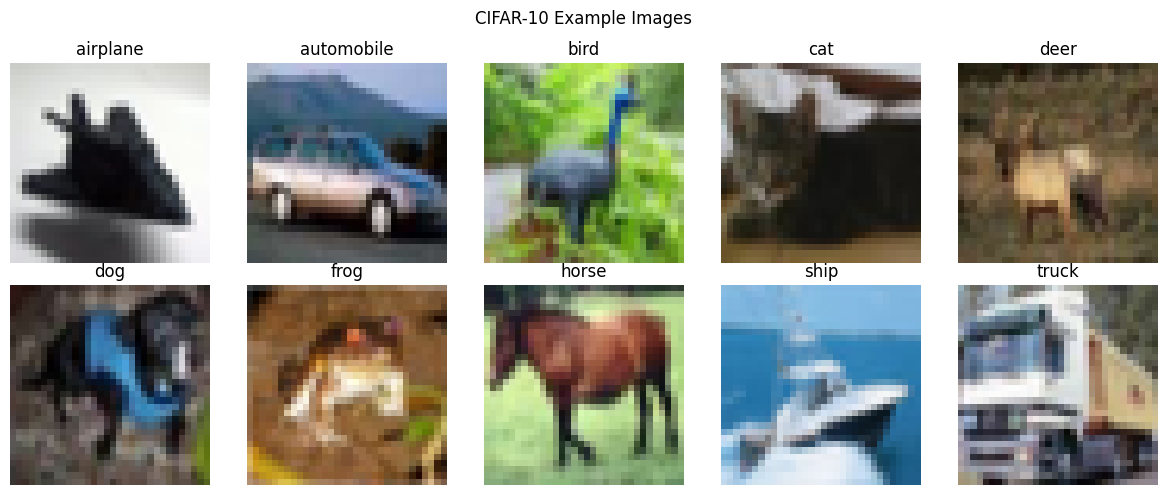
\includegraphics[width=0.85\textwidth]{images/cifar-10-examples.png}
    \caption{One example image per class from the CIFAR-10 training set.}
    \label{fig:cifar10-examples}
\end{figure}

\begin{figure}[h]
    \centering
    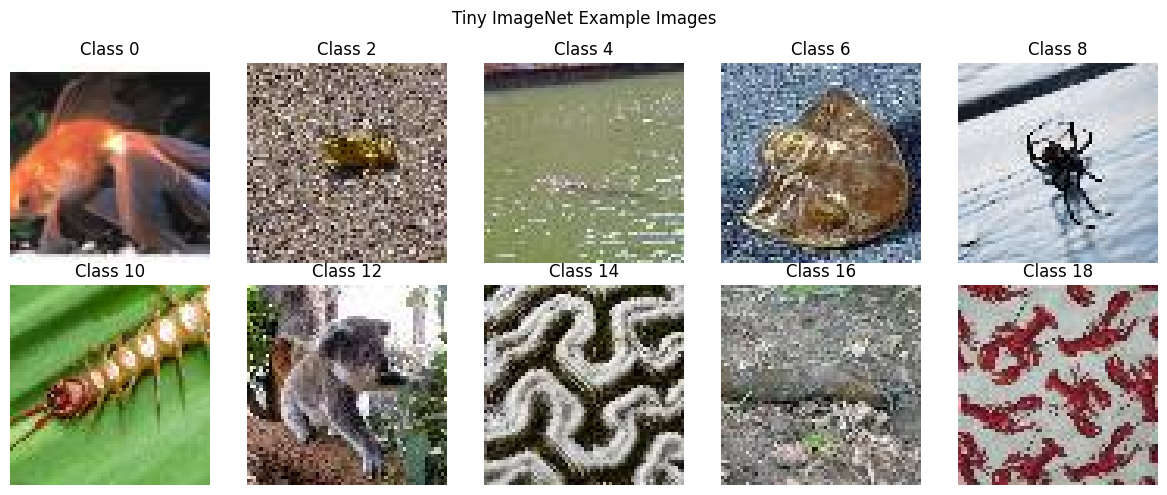
\includegraphics[width=0.85\textwidth]{images/tiny_image_examples.png}
    \caption{Example images from the Tiny ImageNet-200 validation set.}
    \label{fig:tiny-examples}
\end{figure}

\subsection{Training and Testing Performance}

\textbf{DCAE (Task 1).} Figure~\ref{fig:dcae-loss} shows the training and validation loss curves over 50 epochs. Both losses decrease rapidly in the first 10 epochs and continue to converge smoothly, with final values of 0.002352 (train) and 0.002246 (test). The close agreement between training and test loss indicates no significant overfitting.

\begin{figure}[h]
    \centering
    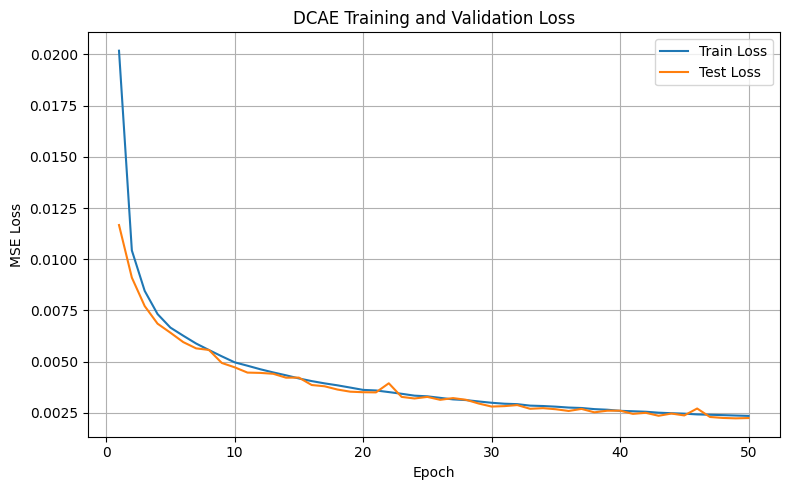
\includegraphics[width=0.75\textwidth]{images/dcae_training_val_loss.png}
    \caption{DCAE training and validation MSE loss over 50 epochs on CIFAR-10.}
    \label{fig:dcae-loss}
\end{figure}

\textbf{VAE (Task 2).} Figure~\ref{fig:vae-loss} shows the ELBO-based training and validation loss curves over 30 epochs. The loss decreases from approximately 425 (epoch 1) to 313.62 (train) and 311.91 (val) at epoch 30. The curves remain closely matched, indicating stable optimization without overfitting.

\begin{figure}[h]
    \centering
    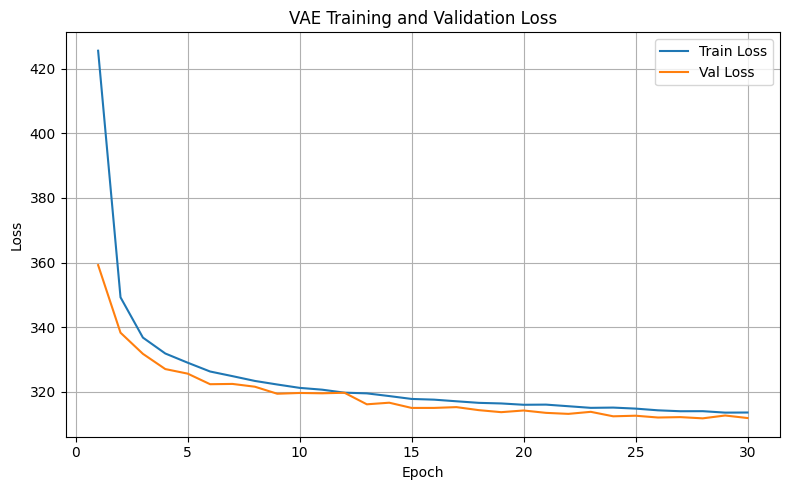
\includegraphics[width=0.75\textwidth]{images/VAE_train_val_loss.png}
    \caption{VAE training and validation ELBO loss over 30 epochs on Tiny ImageNet-200.}
    \label{fig:vae-loss}
\end{figure}

\textbf{DCGAN (Task 2).} Figure~\ref{fig:dcgan-loss} shows the generator and discriminator losses over 30 epochs. The generator loss rises steadily from 4.02 to 5.08, while the discriminator loss oscillates around 0.50--0.58 through the first 13 epochs, then begins a more substantial decline starting at epoch 14 (0.45) and epoch 15 (0.38), ultimately reaching 0.18 by epoch 30. Visually, the discriminator curve barely trends downward relative to the scale of the generator's rise. This pattern is a hallmark of adversarial training imbalance: the discriminator becomes progressively better at rejecting fake images, continuously pushing the generator's loss upward, while the generator fails to keep pace within the 30-epoch budget.

\begin{figure}[h]
    \centering
    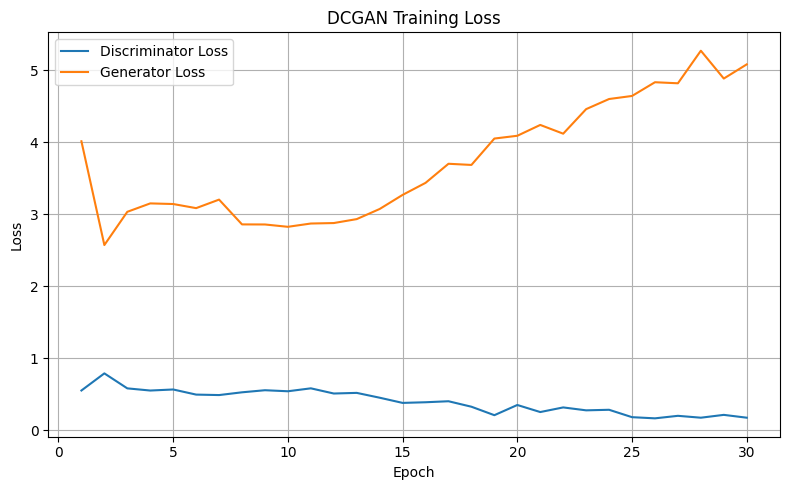
\includegraphics[width=0.75\textwidth]{images/DCGAN_training_loss.png}
    \caption{DCGAN generator and discriminator losses over 30 epochs on Tiny ImageNet-200.}
    \label{fig:dcgan-loss}
\end{figure}

\subsection{Quantitative Evaluation}

Table~\ref{tab:metrics} summarizes the quantitative results for all three models. The DCAE achieves the best reconstruction metrics owing to its deterministic bottleneck and the relative simplicity of CIFAR-10. The VAE reconstruction quality is lower due to the KL regularization penalty, which sacrifices some reconstruction sharpness to maintain a structured latent space. DCGAN metrics are measured against nearest real validation images rather than ground-truth reconstructions, so the higher MSE and lower SSIM reflect the generation gap rather than reconstruction error per se.

\begin{table}[h]
    \centering
    \caption{Quantitative reconstruction and generation quality. $^\dagger$DCGAN values are nearest-neighbor metrics comparing generated images to real validation images, not reconstruction of existing images.}
    \begin{tabular}{lccc}
        \toprule
        \textbf{Model} & \textbf{Task} & \textbf{MSE} & \textbf{SSIM} \\
        \midrule
        DCAE (reconstruction)  & 1 (CIFAR-10)           & 0.002241 $\pm$ 0.001216 & 0.9013 $\pm$ 0.0422 \\
        VAE (reconstruction)   & 2 (Tiny ImageNet-200)  & 0.019281 $\pm$ 0.009069 & 0.3580 $\pm$ 0.1273 \\
        VAE (generated)$^\dagger$       & 2 (Tiny ImageNet-200)  & 0.039263 $\pm$ 0.010706 & 0.1913 $\pm$ 0.0792 \\
        DCGAN (generated)$^\dagger$     & 2 (Tiny ImageNet-200)  & 0.067519 $\pm$ 0.025587 & 0.0936 $\pm$ 0.0549 \\
        \bottomrule
    \end{tabular}
    \label{tab:metrics}
\end{table}

\subsection{Qualitative Evaluation}

\subsubsection{Task 1 --- DCAE Reconstruction}

Figure~\ref{fig:dcae-recon} shows 10 test images paired with their reconstructions. The results are qualitatively strong: object shapes, dominant colors, and spatial layouts are faithfully preserved, and the reconstructions are clearly recognizable as the correct class in all cases. Some fine-grained texture detail is softened, as is typical of MSE-trained autoencoders, but the overall fidelity is high and consistent with the quantitative SSIM of 0.90.

\begin{figure}[h]
    \centering
    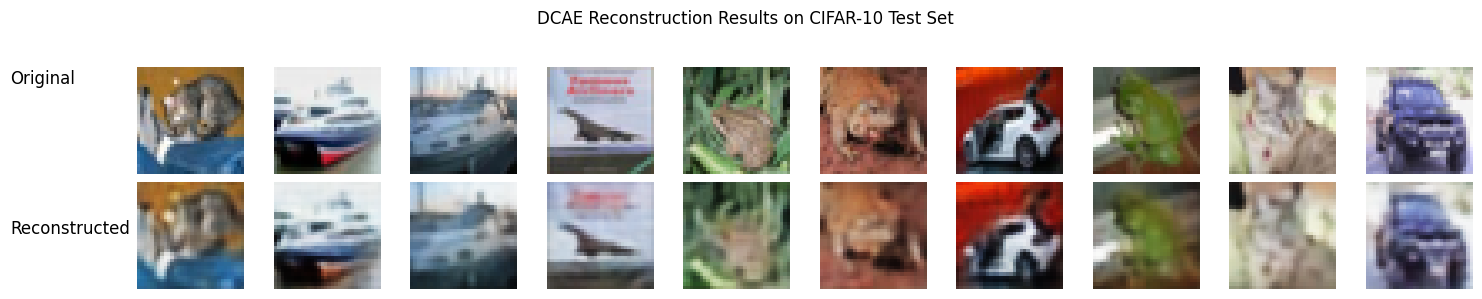
\includegraphics[width=\textwidth]{images/DCAE_original_reconstructed.png}
    \caption{DCAE reconstruction results on the CIFAR-10 test set. Top row: original images. Bottom row: reconstructed images.}
    \label{fig:dcae-recon}
\end{figure}

\subsubsection{Task 1 --- t-SNE Visualization}

Figure~\ref{fig:tsne-pca} shows the t-SNE visualization of the 10-dimensional PCA embeddings for 10,000 randomly sampled images, colored by ground-truth labels (left) and K-means cluster assignments (right).

\begin{figure}[h]
    \centering
    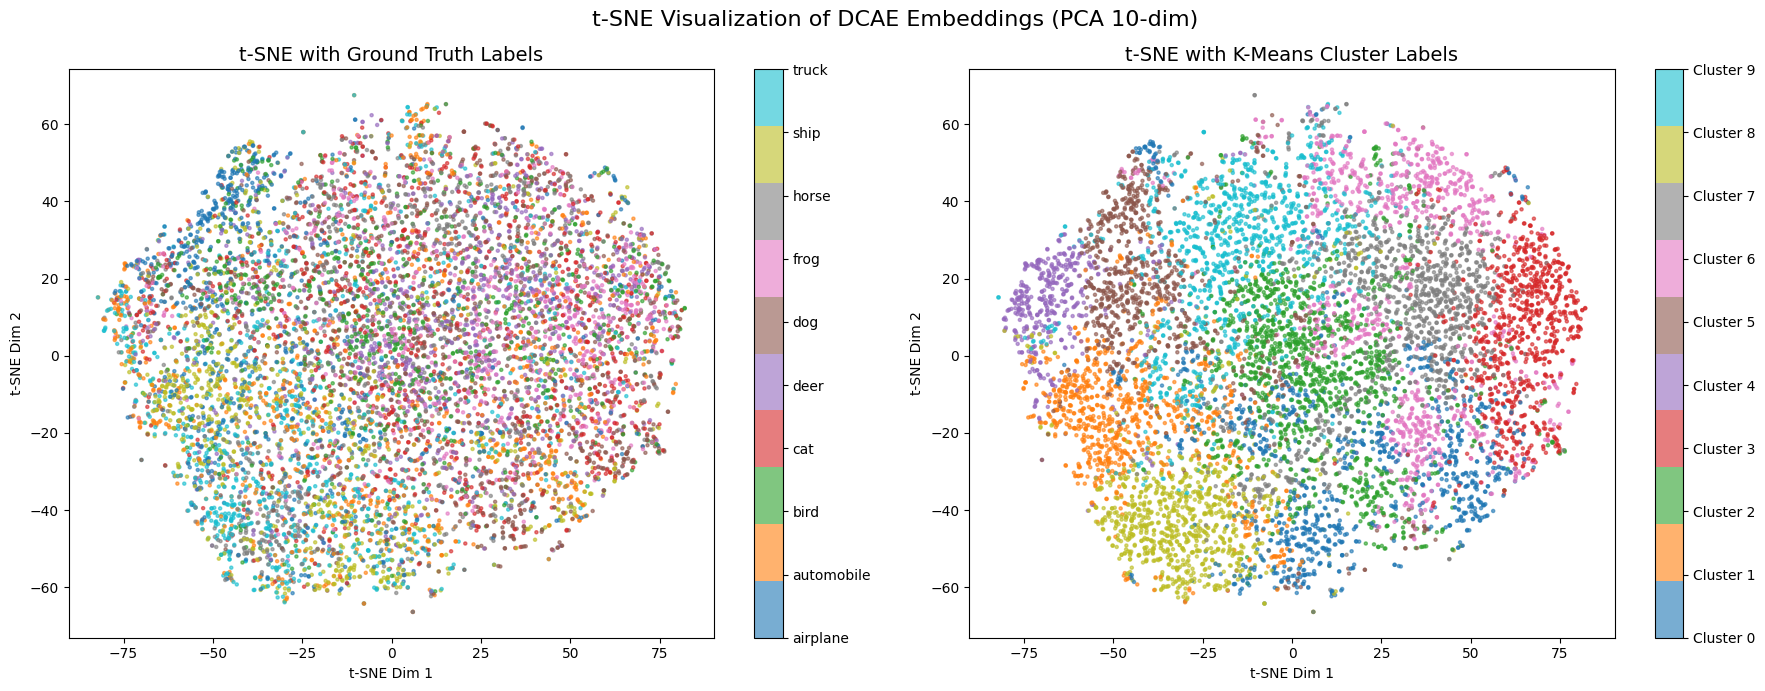
\includegraphics[width=\textwidth]{images/pca-clusters.png}
    \caption{t-SNE visualization of DCAE embeddings (PCA-reduced to 10 dims). Left: ground-truth class labels. Right: K-means cluster labels ($k=10$).}
    \label{fig:tsne-pca}
\end{figure}

The ground-truth-colored plot reveals no apparent spatial pattern: the 10 class colors are thoroughly intermixed across the 2D embedding, indicating that the DCAE latent space (as projected through 10 PCA components) does not naturally separate semantic classes. This is expected given that only 42.64\% of the variance is retained after PCA reduction, and that the DCAE is trained purely on pixel reconstruction without any class-discriminative signal. By contrast, the K-means plot shows well-defined, spatially coherent regions by construction — but these clusters do not correspond cleanly to the ground-truth categories.

Table~\ref{tab:clustering} quantifies the alignment between K-means assignments and ground-truth labels. The ARI of 0.046 and NMI of 0.088 are both close to zero, confirming near-chance agreement between cluster assignments and true classes. The clustering accuracy of 22.57\% (random chance = 10\%) indicates that the K-means clusters capture some coarse visual structure, but the overall alignment is weak — consistent with the intermixed t-SNE visualization.

\begin{table}[h]
    \centering
    \caption{K-means clustering alignment with ground-truth labels on CIFAR-10 (all 60,000 images, $k=10$).}
    \begin{tabular}{lcc}
        \toprule
        \textbf{Metric} & \textbf{Value} & \textbf{Interpretation} \\
        \midrule
        Adjusted Rand Index (ARI)        & 0.0458 & 0 = chance, 1 = perfect \\
        Normalized Mutual Information (NMI) & 0.0875 & 0 = no overlap, 1 = perfect \\
        Clustering Accuracy (Hungarian)  & 22.57\% & random chance = 10\% \\
        \bottomrule
    \end{tabular}
    \label{tab:clustering}
\end{table}

\subsubsection{Task 2 --- Generated Images}

Unlike the VAE and DCAE, the DCGAN has no encoder and therefore cannot reconstruct a given input image; its only output mode is unconditional generation from a noise vector. Quantitative reconstruction metrics are consequently not applicable to the DCGAN, and the nearest-neighbor MSE/SSIM reported in Table~\ref{tab:metrics} serve as a generation-quality proxy rather than a reconstruction score.

Figures~\ref{fig:vae-gen} and~\ref{fig:dcgan-gen} show $8\times8$ grids of images sampled from the VAE and DCGAN decoders, respectively. The VAE-generated images (Figure~\ref{fig:vae-gen}) are heavily blurred and show very little coherent structure: no recognizable objects are discernible, and the samples lack the spatial organization seen even in the VAE reconstructions. This is a known failure mode of MSE-trained decoders when sampling from regions of the prior not covered by the posterior. The DCGAN-generated images (Figure~\ref{fig:dcgan-gen}) are also not recognizable as any specific class, but they exhibit more global coherence — structured color gradients, rough edge-like patterns, and regional contrast — suggesting the generator has captured low-level image statistics even if it has not yet learned to synthesize meaningful objects after 30 epochs.

\begin{figure}[h]
    \centering
    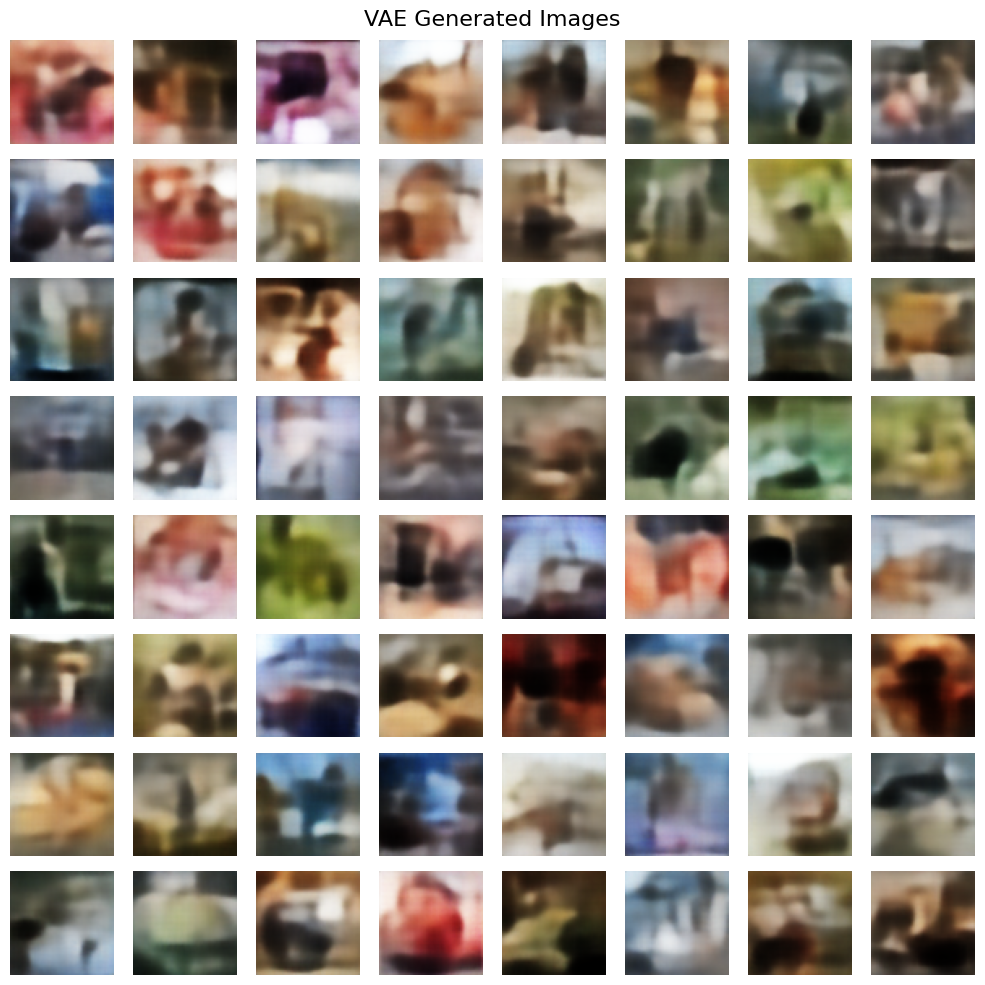
\includegraphics[width=0.75\textwidth]{images/VAE_generated_images.png}
    \caption{Images generated by randomly sampling $\mathbf{z} \sim \mathcal{N}(\mathbf{0}, \mathbf{I})$ from the trained VAE decoder.}
    \label{fig:vae-gen}
\end{figure}

\begin{figure}[h]
    \centering
    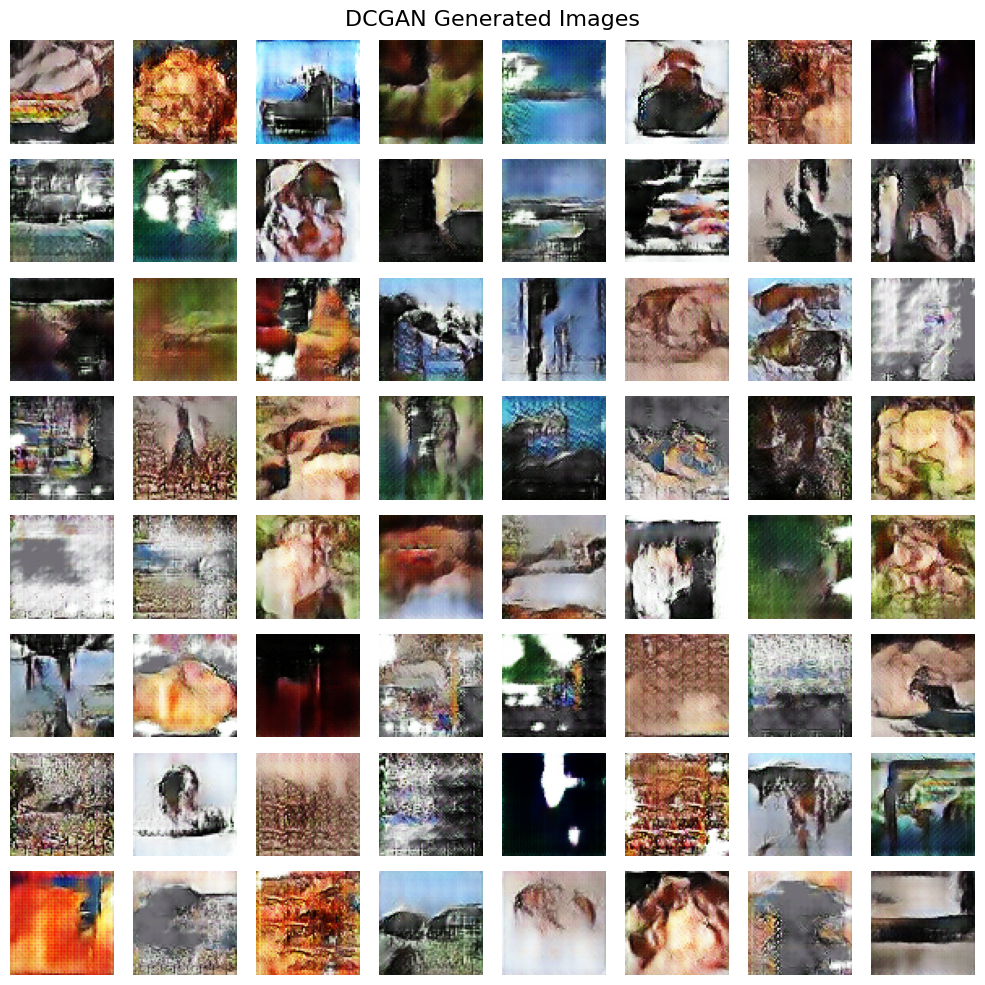
\includegraphics[width=0.75\textwidth]{images/DCGAN_generated_images.png}
    \caption{Images generated by the DCGAN generator from fixed noise vectors at epoch 30.}
    \label{fig:dcgan-gen}
\end{figure}

Figure~\ref{fig:vae-recon} shows VAE reconstructions of validation images. The reconstructions are substantially blurrier than those of the DCAE in Task~1: while the general color palette and rough spatial layout of each image are preserved, object boundaries are heavily smeared and fine details are lost entirely. This is a combined effect of the KL regularization (which diffuses the posterior and reduces per-image specificity), the more demanding $64\times64$ resolution, and the 200-class diversity of Tiny ImageNet.

\begin{figure}[h]
    \centering
    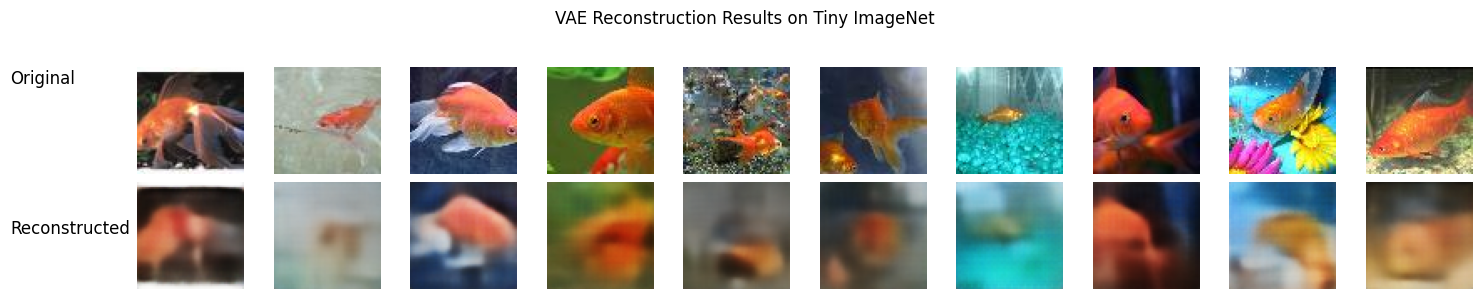
\includegraphics[width=\textwidth]{images/VAE_original_reconstructed.png}
    \caption{VAE reconstruction results on Tiny ImageNet-200 validation images. Top row: original. Bottom row: reconstructed.}
    \label{fig:vae-recon}
\end{figure}

\subsubsection{Task 2 --- t-SNE of Latent Space}

Figure~\ref{fig:tsne-vae-gan} shows t-SNE projections of 5,000 validation images: VAE $\mu$ vectors (left) and DCGAN discriminator features (right), both colored by class label.

\begin{figure}[h]
    \centering
    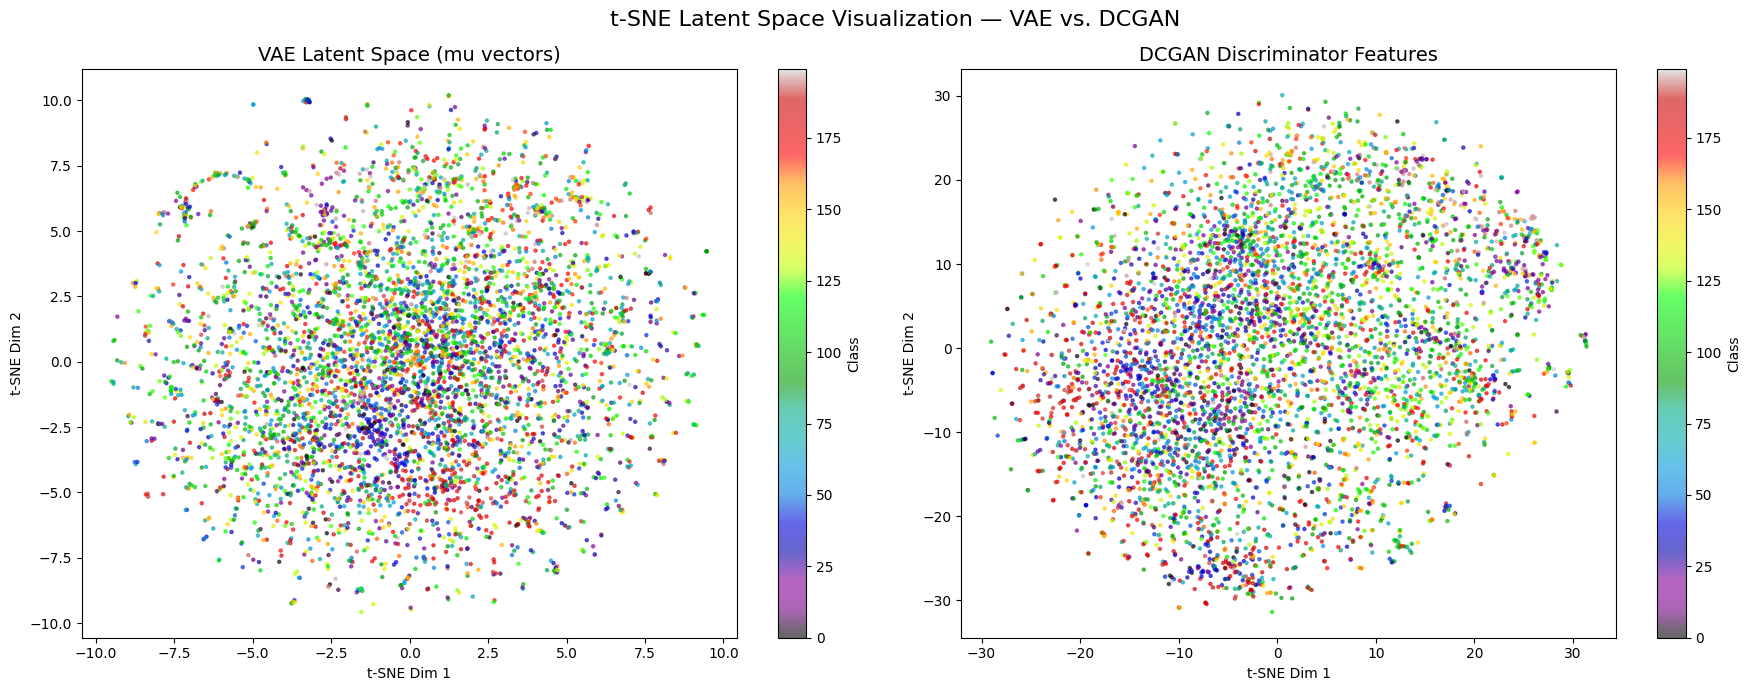
\includegraphics[width=\textwidth]{images/tSNE_VAE_vs_DCGAN.png}
    \caption{t-SNE of latent representations on Tiny ImageNet-200 validation set. Left: VAE $\mu$ vectors ($d=256$). Right: DCGAN discriminator intermediate features ($d=4096$).}
    \label{fig:tsne-vae-gan}
\end{figure}

The VAE latent space (left) shows a small number of clearly identifiable, well-separated clusters, though they are sparse relative to the full 200-class spread. This suggests the VAE's KL regularization does produce some genuine semantic groupings for the most visually distinctive classes, even without any label supervision. The DCGAN discriminator features (right) form denser, more compact blobs overall, but the color coding within those blobs is mixed: classes are not cleanly separated, and the clusters reflect low-level visual texture and color statistics rather than semantic identity. This contrast is expected — the VAE encoder is explicitly trained to produce a structured Gaussian posterior, while the DCGAN discriminator only needs to distinguish real from fake and has no incentive to organize features by class.

\subsection{Comparative Analysis}

Comparing the two generative models, the VAE offers better reconstruction metrics (MSE 0.019 vs.\ 0.068) and more semantically structured latent embeddings, but its randomly sampled images are heavily blurred and incoherent — worse than the DCGAN qualitatively despite the better numbers. The DCGAN's generated images are also not recognizable as any specific object class, but they exhibit more global spatial coherence (structured gradients, regional contrast), suggesting the adversarial objective better preserves low-level image statistics. The divergence between generator and discriminator losses indicates that 30 training epochs are insufficient for convergence on the complex 200-class Tiny ImageNet distribution.

The DCAE significantly outperforms both generative models in reconstruction quality (SSIM 0.90 vs.\ 0.36 for VAE), benefiting from a deterministic bottleneck, a simpler dataset, and a direct MSE objective. However, the DCAE cannot generate novel images: it is purely a feature extractor and compressor.

\subsection{Limitations and Challenges}

\begin{itemize}
    \item \textbf{Computational constraints.} All models were trained on CPU, which limited the number of epochs (50 for DCAE, 30 for VAE and DCGAN). GPU training would permit longer runs and potentially better convergence, particularly for the DCGAN.
    \item \textbf{DCGAN training instability.} The growing divergence between generator and discriminator losses is a sign of training imbalance. Techniques such as spectral normalization, gradient penalty, or one-sided label smoothing could improve stability.
    \item \textbf{VAE blurriness.} The MSE reconstruction term promotes average-pixel fidelity at the expense of sharpness. Perceptual loss functions or VQ-VAE discrete codebooks could mitigate this.
    \item \textbf{PCA variance retention.} Only 42.64\% of the variance in the 512-dimensional DCAE embeddings is retained in the 10-dimensional PCA projection, which limits the quality of subsequent K-means clustering. The individual explained-variance ratios for the top 10 components are 12.3\%, 6.1\%, 4.9\%, 3.7\%, 3.4\%, 3.1\%, 2.5\%, 2.4\%, 2.4\%, and 2.0\%, indicating rapid drop-off: retaining 50 or 100 components before K-means would substantially increase variance coverage and likely improve cluster--class alignment, at the cost of slower K-means convergence.
    \item \textbf{No learning rate scheduling.} All three models use a fixed learning rate throughout training. A cosine annealing or step decay schedule would allow larger initial learning rates for rapid early-epoch progress while reducing the rate in later epochs to fine-tune the weights. For the DCAE (50 epochs) and DCGAN (30 epochs) in particular, the flat loss curves in the final 10–15 epochs suggest the optimizer has stalled at a learning rate that is too high for fine-grained updates.
    \item \textbf{Dataset complexity.} Tiny ImageNet-200 has 200 classes with fine-grained diversity; both generative models would benefit from more training epochs and a larger model capacity.
\end{itemize}

%--------------------------------------------------------
% 5. Conclusion and Future Work
%--------------------------------------------------------
\section{Conclusion and Future Work}

This work demonstrated the implementation and evaluation of three deep unsupervised models. The DCAE on CIFAR-10 achieved high-quality reconstruction (SSIM 0.90); however, the t-SNE visualization revealed limited class separation in the latent space after PCA reduction, consistent with the unsupervised training objective. On Tiny ImageNet-200, the VAE outperformed the DCGAN on quantitative reconstruction metrics and latent-space organization, while the DCGAN produced sharper but less consistent generated images.

Key takeaways are: (1) deterministic autoencoders are most effective when the goal is reconstruction rather than generation; (2) the VAE's structured latent space enables smoother sampling and better latent-space visualization than GAN-based features; (3) DCGAN training requires careful tuning and more epochs to fully exploit its capacity on complex, multi-class datasets.

Future directions include: replacing the MSE loss in the VAE with a perceptual or adversarial loss to sharpen generated images; applying VQ-VAE or diffusion models for higher-fidelity synthesis; investigating progressive-growing GANs or StyleGAN2 for stable high-resolution generation; increasing PCA components before K-means to improve clustering accuracy; and extending the evaluation to include Fréchet Inception Distance (FID) for a more perceptually aligned generation quality metric.

%--------------------------------------------------------
% References
%--------------------------------------------------------
\begin{thebibliography}{10}

\bibitem{hinton2006}
G. E. Hinton and R. R. Salakhutdinov,
``Reducing the dimensionality of data with neural networks,''
\textit{Science}, vol.\ 313, no.\ 5786, pp.\ 504--507, 2006.

\bibitem{vae2013}
D. P. Kingma and M. Welling,
``Auto-encoding variational Bayes,''
in \textit{Proc. Int. Conf. Learning Representations (ICLR)}, 2014.
arXiv:1312.6114.

\bibitem{gan2014}
I. Goodfellow, J. Pouget-Abadie, M. Mirza, B. Xu, D. Warde-Farley, S. Ozair, A. Courville, and Y. Bengio,
``Generative adversarial nets,''
in \textit{Advances in Neural Information Processing Systems (NeurIPS)}, vol.\ 27, 2014.

\bibitem{dcgan2015}
A. Radford, L. Metz, and S. Chintala,
``Unsupervised representation learning with deep convolutional generative adversarial networks,''
in \textit{Proc. ICLR}, 2016.
arXiv:1511.06434.

\bibitem{cifar10}
A. Krizhevsky,
``Learning multiple layers of features from tiny images,''
Tech. Report, University of Toronto, 2009.

\bibitem{tinyimagenet}
Y. Le and X. Yang,
``Tiny ImageNet visual recognition challenge,''
CS231N Class Project Report, Stanford University, 2015.

\bibitem{tsne2008}
L. van der Maaten and G. Hinton,
``Visualizing data using t-SNE,''
\textit{J. Mach. Learn. Res.}, vol.\ 9, pp.\ 2579--2605, 2008.

\bibitem{ssim2004}
Z. Wang, A. C. Bovik, H. R. Sheikh, and E. P. Simoncelli,
``Image quality assessment: From error visibility to structural similarity,''
\textit{IEEE Trans. Image Process.}, vol.\ 13, no.\ 4, pp.\ 600--612, Apr.\ 2004.

\bibitem{fid2017}
M. Heusel, H. Ramsauer, T. Unterthiner, B. Nessler, and S. Hochreiter,
``GANs trained by a two time-scale update rule converge to a local Nash equilibrium,''
in \textit{Advances in Neural Information Processing Systems (NeurIPS)}, vol.\ 30, 2017.

\bibitem{adam2014}
D. P. Kingma and J. Ba,
``Adam: A method for stochastic optimization,''
in \textit{Proc. ICLR}, 2015.
arXiv:1412.6980.

\bibitem{batchnorm2015}
S. Ioffe and C. Szegedy,
``Batch normalization: Accelerating deep network training by reducing internal covariate shift,''
in \textit{Proc. Int. Conf. Machine Learning (ICML)}, pp.\ 448--456, 2015.

\end{thebibliography}

%--------------------------------------------------------
% Appendix
%--------------------------------------------------------
\appendix
\section{Hyperparameter Tables}

\begin{table}[h]
    \centering
    \caption{DCAE hyperparameters (Task 1).}
    \begin{tabular}{ll}
        \toprule
        \textbf{Hyperparameter} & \textbf{Value} \\
        \midrule
        Latent dimension          & 512 \\
        Input size                & $3 \times 32 \times 32$ \\
        Encoder channels          & 3, 32, 64, 128, 256 \\
        Conv kernel / stride / pad & $3\times3$ / 2 / 1 \\
        Decoder transposed conv   & $3\times3$ / 2 / 1 (output pad 1) \\
        Batch normalization       & Yes (all conv layers) \\
        Encoder activation        & ReLU \\
        Decoder activation        & ReLU (hidden), Sigmoid (output) \\
        Loss function             & MSE \\
        Optimizer                 & Adam \\
        Learning rate             & $1\times10^{-3}$ \\
        Batch size                & 128 \\
        Epochs                    & 50 \\
        Total parameters          & 1,828,099 \\
        \bottomrule
    \end{tabular}
\end{table}

\begin{table}[h]
    \centering
    \caption{Convolutional VAE hyperparameters (Task 2).}
    \begin{tabular}{ll}
        \toprule
        \textbf{Hyperparameter} & \textbf{Value} \\
        \midrule
        Latent dimension             & 256 \\
        Input size                   & $3 \times 64 \times 64$ \\
        Encoder channels             & 3, 32, 64, 128, 256 \\
        Conv kernel / stride / pad   & $4\times4$ / 2 / 1 \\
        Encoder activation           & LeakyReLU (slope 0.2) \\
        Decoder activation           & ReLU (hidden), Sigmoid (output) \\
        Loss function                & MSE reconstruction + KL divergence \\
        Optimizer                    & Adam \\
        Learning rate                & $1\times10^{-3}$ \\
        Batch size                   & 128 \\
        Epochs                       & 30 \\
        Total parameters             & 4,531,779 \\
        \bottomrule
    \end{tabular}
\end{table}

\begin{table}[h]
    \centering
    \caption{DCGAN hyperparameters (Task 2).}
    \begin{tabular}{ll}
        \toprule
        \textbf{Hyperparameter} & \textbf{Value} \\
        \midrule
        Noise dimension                  & 100 \\
        Input image size                 & $3 \times 64 \times 64$ \\
        Generator channels               & 256, 128, 64, 32, 3 \\
        Discriminator channels           & 3, 32, 64, 128, 256 \\
        Conv kernel / stride / pad       & $4\times4$ / 2 / 1 \\
        Generator activation             & ReLU (hidden), Tanh (output) \\
        Discriminator activation         & LeakyReLU 0.2 \\
        Weight initialization            & $\mathcal{N}(0, 0.02)$ \\
        Loss function                    & BCEWithLogitsLoss \\
        Optimizer (G and D)              & Adam \\
        Learning rate                    & $2\times10^{-4}$ \\
        Adam $\beta_1$ / $\beta_2$       & 0.5 / 0.999 \\
        Batch size                       & 128 \\
        Epochs                           & 30 \\
        Generator parameters             & 1,104,035 \\
        Discriminator parameters         & 695,137 \\
        \bottomrule
    \end{tabular}
\end{table}

\begin{table}[h]
    \centering
    \caption{PCA and clustering pipeline (Task 1).}
    \begin{tabular}{ll}
        \toprule
        \textbf{Parameter} & \textbf{Value} \\
        \midrule
        Input embedding dimension      & 512 \\
        PCA output dimension           & 10 \\
        Total PCA variance retained    & 42.64\% (top 5 shown below) \\
        Top-5 PCA explained variances  & 12.28\%, 6.06\%, 4.90\%, 3.75\%, 3.43\% \\
        K-means clusters ($k$)         & 10 \\
        K-means \texttt{n\_init}       & 10 \\
        t-SNE perplexity               & 30 \\
        t-SNE subsample size           & 10,000 \\
        \bottomrule
    \end{tabular}
\end{table}

\end{document}
